\section{Soluções Sólidas}\label{sec:LABEL_CHP_1_SEC_A}


Segundo Yeh as ligas metálicas apresentam três possíveis configurações no seu estado sólido, são elas: compostos intermetálicos, fases elementares e soluções sólidas. Fases elementares apresentam um único componente em sua matriz, isto é, é o metal sem nenhuma impureza. Seguindo pelos compostos intermetálicos, onde geralmente são formados por dois ou mais elementos além de possuir estrutura bem definida e composição estequiométrica. Por fim temos a solução sólida, os átomos são distribuídos de maneira aleatória e uniforme no interior do sólido, e os sítios da rede cristalina são compartilhados de maneira aleatória. \cite{yeh2013alloy}

A solução sólida é a combinação de dois ou mais sólidos cristalinos que são capazes de coexistir em um novo sólido cristalino ou em uma nova rede cristalina (Figura \ref{fig:solucao-solida}). Assim como os líquidos, os sólidos apresentam diferentes graus de solubilidade mútua. Sendo assim, dependendo das propriedades químicas e da estrutura cristalina de cada elemento, a forma final da rede cristalina da mistura será determinada pela organização e a ligação de cada elemento. Essa solução sólida pode ser substitucional, isto é, quando um átomo ocupa um sítio vazio na rede (uma lacuna/vacância) \cite{britannicaSS}. A solução sólida também pode ser intersticial, ou seja, os átomos de impureza preenchem os vazios ou interstícios que existem entre os átomos hospedeiros.

\begin{figure}[ht]
    \centering
    
    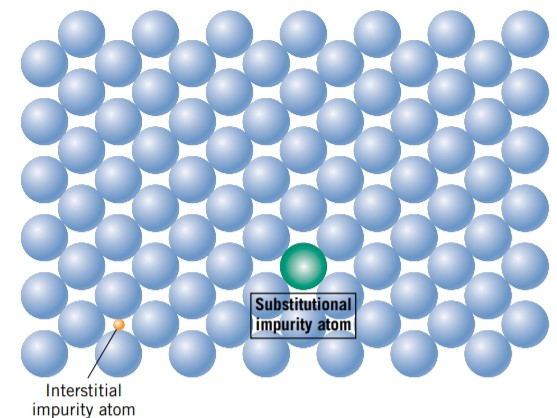
\includegraphics[width=7.7cm,height=5.5cm]{solucao-solida.jpg}
    \caption{Representação de impurezas substitucionais e intersticiais. Adaptado de \cite{callister2011materials}}
    \label{fig:solucao-solida}
\end{figure}

\pagebreak

Existem várias características que determinam o grau em que um elemento pode se solubilizar na rede \cite{callister2011materials}, são essas : 

\begin{itemize}
   \item Fator do tamanho atômico: Quando a diferença dos raios atômicos entre os dois tipos de átomos for menor que aproximadamente 15\%. Ao contrário os átomos com muita diferença no raio atômico que ocuparem as lacunas irão criar distorções substanciais na rede e uma nova fase irá se formar.
    \item Estrutura cristalina: Para que a solubilidade sólida seja considerável, as estruturas cristalinas dos metais de ambos os tipos de átomos devem ser as mesmas.
    \item Eletronegatividade: Quanto maior a eletronegatividade entre dois elementos, isto é, quanto mais eletropositivo for um elemento e mais eletronegativo for o outro, maior a probabilidade e formação de um composto intermetálico. Sendo assim, quanto menor a diferença de eletronegatividade entre dois componentes, maior a possibilidade de formar solução sólida.
    \item Valências: Sendo iguais todos os demais fatores, um metal apresentará maior tendência de dissolver um outro metal de maior valência.
\end{itemize}

Se esses três fatores abordados anteriormente não forem muito semelhantes, existe apenas uma solubilidade limitada. Este cenário pode ser descrito da seguinte maneira, em um solvente puro, alguns átomos são removidos e substituídos por átomos de soluto gradativamente, para aumentar a concentração de soluto. Eventualmente, no entanto, um nível de concentração máxima de soluto é atingido, e alguns átomos começam a ser rejeitados. Eles podem se agrupar para formar um pequeno cristal próprio, talvez com alguns átomos de solvente dissolvidos nele, ou reagir com alguns dos átomos de solvente para formar uma fase da estrutura do cristal diferente daquela de qualquer metal puro (ou seja, um metal intermetálico composto). No diagrama de fases as fases nas extremidades são denominadas terminal ou primária, e no centro do diagrama são denominadas as fases intermediárias. 

Soluções sólidas são definidas como substitucionais quando os elementos do soluto ocupam locais da rede que pertencem aos elementos do solvente, como no caso  do Níquel e Cobre que possuem apenas 2.5\% de diferença de raio atômico, apenas um elétron de diferença na camada de valência, e ambos apresentam estrutura cúbica de face centrada. Essa proximidade entre os dois elementos permite uma total solubilidade. Os átomos de níquel ocupam os locais da rede dos átomos de cobre e vice-versa indiscriminadamente para todas as composições, pode-se dizer que ambos formam uma série contínua de soluções sólidas. O diagrama de fases da liga binária Cu-Ni pode ser observado na Figura \ref{fig:diagrama-ni-cu}.

\pagebreak

\begin{figure}[ht]
    \centering
    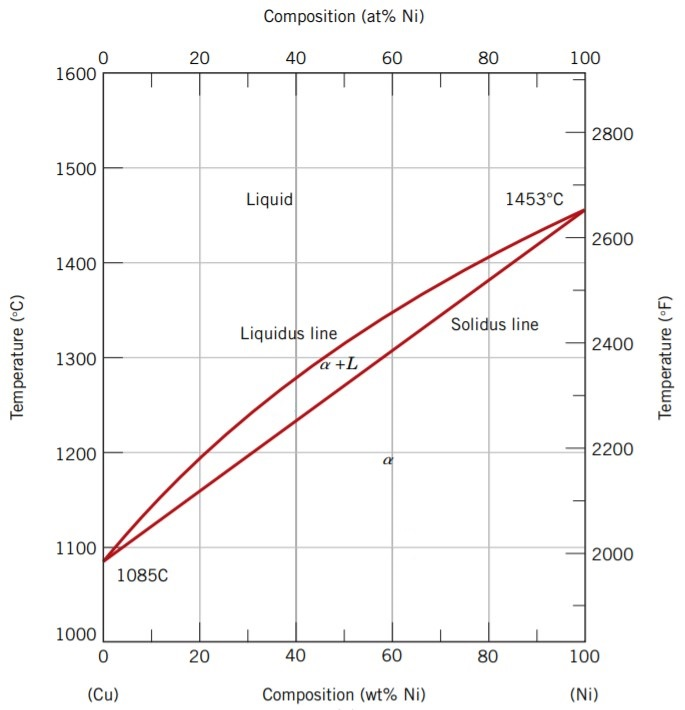
\includegraphics[height=8cm]{diagram-ni-cu.jpg} 
    \caption{Diagrama de fases Cobre-Níquel. Adaptado de \cite{callister2011materials} }
    \label{fig:diagrama-ni-cu}
\end{figure}


Algumas ligas metálicas em altas temperaturas apresentam solubilidade sólida completa, e quando submetidas a baixas temperaturas formam compostos intermetálicos. Porém, na grande maioria dos diagramas de fases de ligas metálicas conhecidas, o fenômeno de solubilidade sólida é relativamente restrito a pequenos intervalos de composição \cite{massalski1996structure}.

Soluções sólidas pode ser aleatórias, quando os elementos se distribuem na rede sem localização preferencial, ou podem ser ordenadas, quando determinados átomos diferentes apresentam certa afinidade. Se átomos da mesma natureza apresentarem afinidade, a formação de aglomerados tende a ocorrer, os quais podem distribuir de maneira ordenada ou aleatória\cite{massalski1996structure}. Exemplos de categorias de soluções sólidas estão demonstrados na Figura \ref{fig:modelo-ss} .

\begin{figure}[ht]
    \centering
    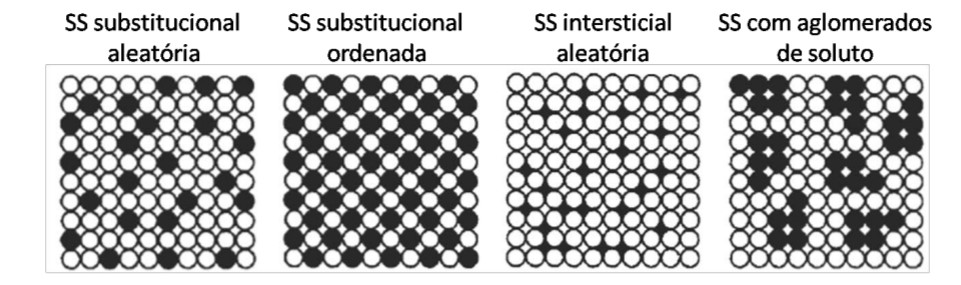
\includegraphics[width=12cm]{modelo-ss.jpg} 
    \caption{ Modelos esquemáticos de soluções sólidas. Adaptado de \cite{massalski1996structure}}
    \label{fig:modelo-ss}
\end{figure}
